\documentclass[10pt]{article}
\usepackage[polish]{babel}
\usepackage[utf8]{inputenc}
\usepackage[T1]{fontenc}
\usepackage{graphicx}
\usepackage[export]{adjustbox}
\graphicspath{ {./images/} }
\usepackage{amsmath}
\usepackage{amsfonts}
\usepackage{amssymb}
\usepackage[version=4]{mhchem}
\usepackage{stmaryrd}

\title{Zestaw 2 }

\author{}
\date{}


\begin{document}
\maketitle
\begin{center}

\includegraphics[max width=\textwidth]{2024_11_21_388519d38d11b6d14f67g-1}
\end{center}

\begin{enumerate}
  \item Dany jest 100-kąt foremny. Wybrano 51 jego wierzchołków. Wykaż, że wśród wybranych punktów istnieją trzy będące wierzchołkami trójkąta prostokątnego równoramiennego.
  \item Wyznacz dwie ostatnie cyfry zapisu dziesiętnego liczby
\end{enumerate}

\[
2^{5^{1}}+2^{5^{2}}+2^{5^{3}}+\cdots+2^{5^{2017}}+2^{5^{2018}}
\]

\begin{enumerate}
  \setcounter{enumi}{2}
  \item W trójkącie ABC punkt I jest środkiem okręgu wpisanego, zaś punkt D różnym od A punktem wspólnym prostej Al i okręgu opisanego na trójkącie \(A B C\). Udowodnij, że odcinki BD, CD i DI są jednakowej długości.\\
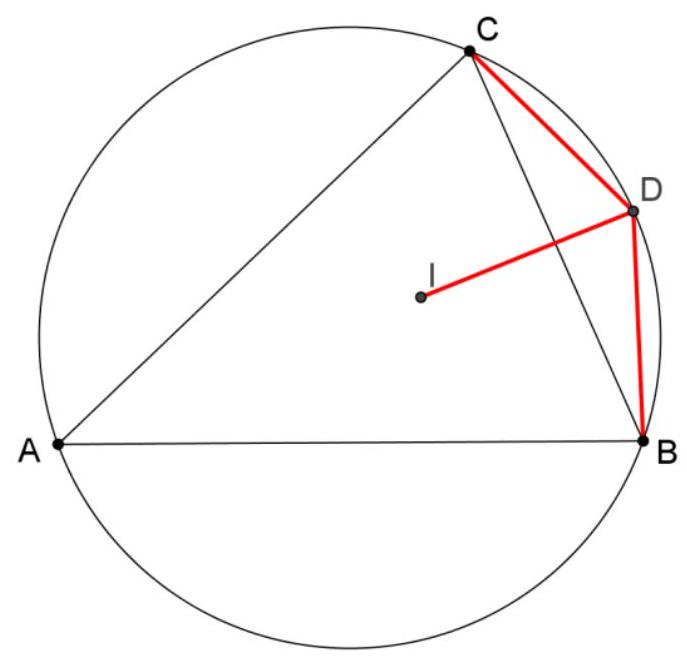
\includegraphics[max width=\textwidth, center]{2024_11_21_388519d38d11b6d14f67g-1(1)}
\end{enumerate}

\end{document}